\documentclass[tikz,border=8pt]{standalone}

\usepackage{amsmath} % needed for \matrix
\usetikzlibrary{matrix,positioning,calc}

\begin{document}
    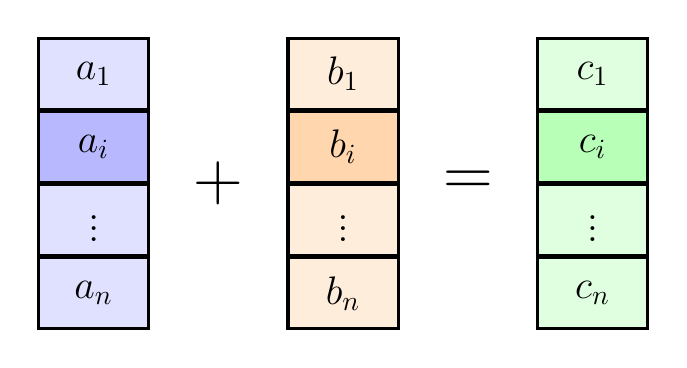
\begin{tikzpicture}[
        font=\Large,
        cell/.style={draw, very thick, minimum width=14mm, minimum height=9mm, align=center},
        vecA/.style={cell, fill=blue!12},
        vecB/.style={cell, fill=orange!14},
        vecC/.style={cell, fill=green!12},
        hiA/.style={cell, fill=blue!28},
        hiB/.style={cell, fill=orange!32},
        hiC/.style={cell, fill=green!28},
        op/.style={font=\Huge}
    ]

% --- Vector a (just the grid) ---
        \matrix (A) [matrix of nodes, nodes in empty cells, row sep=-\pgflinewidth, column sep=-\pgflinewidth] {
            \node[vecA] {$a_{1}$}; \\
            \node[hiA]  {$a_{i}$}; \\
            \node[vecA] {$\vdots$}; \\
            \node[vecA] {$a_{n}$}; \\
        };

% --- Plus sign (close) ---
        \node[op, right=3mm of A] (plus) {$+$};

% --- Vector b (just the grid) ---
        \matrix (B) [matrix of nodes, nodes in empty cells, row sep=-\pgflinewidth, column sep=-\pgflinewidth, right=3mm of plus] {
            \node[vecB] {$b_{1}$}; \\
            \node[hiB]  {$b_{i}$}; \\
            \node[vecB] {$\vdots$}; \\
            \node[vecB] {$b_{n}$}; \\
        };

% --- Equals sign (close) ---
        \node[op, right=3mm of B] (eq) {$=$};

% --- Vector c (just the grid) ---
        \matrix (C) [matrix of nodes, nodes in empty cells, row sep=-\pgflinewidth, column sep=-\pgflinewidth, right=3mm of eq] {
            \node[vecC] {$c_{1}$}; \\
            \node[hiC]  {$c_{i}$}; \\
            \node[vecC] {$\vdots$}; \\
            \node[vecC] {$c_{n}$}; \\
        };

    \end{tikzpicture}
\end{document}